\chapter{Method}
%\thispagestyle{empty}


\section{Performance comparison/Terms}
\Todo{move to results? or at end of method}

Before we can go further and present the methods and results of the experiments
it is necessary to introduce some additional terms. 
Such as metrics to measure their performance.


\paragraph{Mean squared error (MSE)} is an error measurement that
describes the error/noise between an given or measured reference signal $x$
and  and the reconstruction(noisy approximation) $\tilde{x}$ of it.
Mathematically it is defined as the average of the squared error between two
signals.
%The mean squared error is defined as:
\begin{align}
 MSE = \frac{1}{n} \sum_{i=0}^{n} \left( {\lVert x_i -
\tilde{x}_i\rVert^{2}}\right)
\end{align}
We primarily use it for testing dictionary learning convergence and as a
sub term for the measurement described in the next paragraph.

\paragraph{Peak signal-to-noise ration (PSNR)} describes the ratio between the
error/noise affecting a signal/reconstruction and the maximum possible signal
amplitude. It is expressed in a logarithmic decibel scale.
\begin{align}
 PSNR = 20 \cdot \log_{10} \left(\frac{MAX}{\sqrt{MSE}}\right)
\end{align}
Where $MAX$ is the maximum possible value of our signal. For an 8-bit
image it would be 255. For a 32-bit normalized image it would be 1. And $MSE$ is
the mean squared error between a reference signal and its reconstruction. The
PSNR is undefined for zero noise.

The PSNR is primarily used for comparison of the reconstruction quality of
lossy compression algorithms. Typical values for a lossy reconstruction lie in
a range between 30dB and
50dB.\footnote{\url{http://en.wikipedia.org/wiki/Peak_signal-to-noise_ratio}}
%e.g. relevant for de-noise


\paragraph{Bits per pixel (bpp)} 
For the comparison of compression ratio of images another well known practice is
to measure the required \emph{bits per pixel} short bpp. The bbp are calculated
by dividing the raw image data by the image's dimensions. For example an
uncompressed RGB color image with 8-bit of color depth requires 24-bits per
pixel, respectively a gray scale image with 8-bit for a single channel requires
8-bits. While compression algorithms are able to encode multiple pixels with few
coefficient leading to much lower bpp rates.
Looking at other well known compression algorithms such as JPEG or
JPEG 2000 a common ratio is about $\sim1.8$ bits-per-pixel for average
quality compression( JPEG quality of 50) of an natural image. 
\Todo{example image?, lower bit rates, Lewicki estimate for sparse coding}

Besides the raw pixel data, images formats usually contain a certain amount
of extra data from file headers and meta data. Fortunately we can ignore this
for simplification as it is only a few bytes and not being actual pixel data.

\paragraph{Test data}
In addition to the introduced metrics it is common practice to use some image
sets to compare test results of the different algorithms and parameter
configurations. For comparison of the reconstruction quality and compression
quality we use a well known set of standard test images from the \emph{USC-SIPI
Image Database}\footnote{\url{http://sipi.usc.edu/database/}}. They are often
used in image processing for evaluation of compression algorithms. 
Including pictures such as Lena, Mandrill and Peppers.



\section{Signal representation}
\label{sec:signal_representation}
To be able efficiently sparse code images it is necessary to prepare the
image data. As we mainly use sets of color images and graphics we require
to work with multi-channel data. Commonly presented in the three channel RGB
color space. 

%The initial signal data 
%We use an approach to transform our initial signal into other color spaces like
%in JPEG encoding to account natural human reception of color data.
%Experiment ....

%\paragraph{Color space conversion}
\paragraph{Chroma sub-sampling} is used to reduce the amount of data required by
color information while preserving perceptual image quality. 
The human eye is good at sensing small difference in brightness but lacks the
ability exactly differentiate small changes in color. Chroma sub-sampling takes
advantage of this human flaw. First the image gets converted into the $YC_bC_r$
color space, which describes an image in a brightness/luminance (Y) and two
color/chroma components (Cb and Cr). Then the visual more relevant
brightness/luminance channel will be coded in the full resolution while the
color/chroma components can be sub-sampled with only minor loss in perceptual
quality. This procedure, illustrated in fig. \ref{fig:YCbCr}, is one key element
in lossy image compression. 
\begin{figure}[h]
\centering
\subfloat[Y]{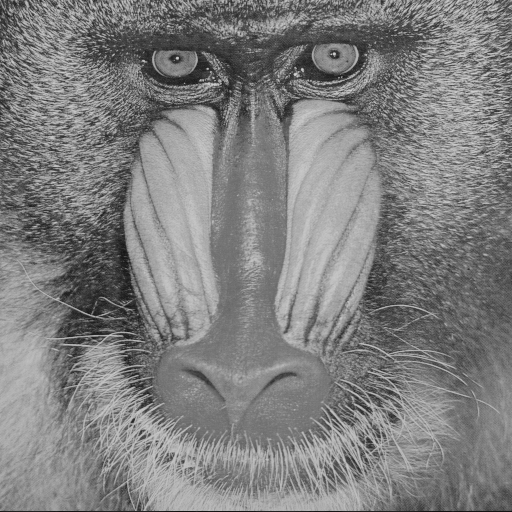
\includegraphics[width =
0.3\textwidth]{images/y.png}}
\hspace{5mm}
\subfloat[Cb]{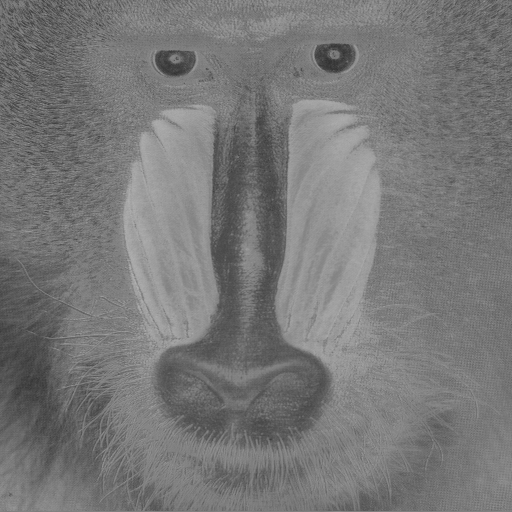
\includegraphics[width =
0.3\textwidth]{images/cb.png}}
\hspace{5mm}
\subfloat[Cr]{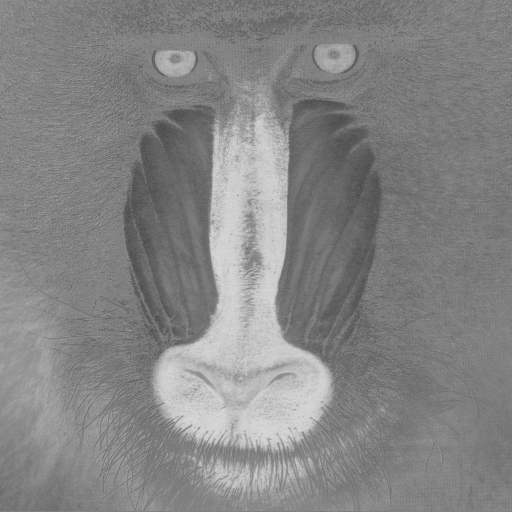
\includegraphics[width =
0.3\textwidth]{images/cr.png}}
\caption{RGB $\rightarrow$ YCbCr}
\label{fig:YCbCr}
\end{figure}
%color space, high/low pass filtering
%\subsection{color/signal representation}


\paragraph{Spartial seperation}

\begin{figure}[h]
\centering
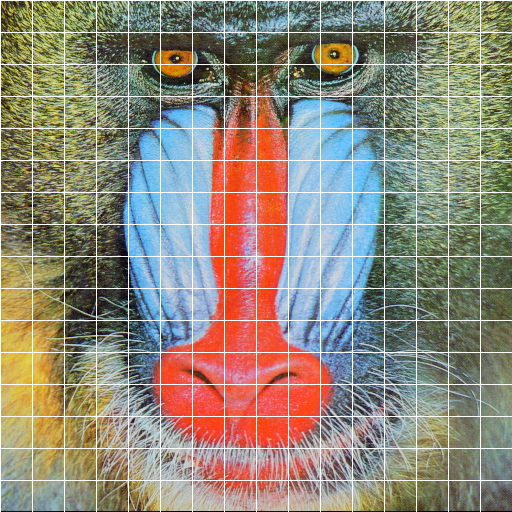
\includegraphics[scale = 0.25]{images/segmentation.png}
\caption{spartial separation}
\label{fig:spartial}
\end{figure}

\section{Sparse coding step}
\subsection{Batch-OMP}
In 2008 Rubinstein et al.\cite{Rubinstein2008} presented the \emph{Batch-OMP}.
The
\prettyref{alg:batchOMP} is a modified version of the
orthogonal-matching-pursuit (\ref{sec:omp}) that can effectively sparse code
multiple signals in parallel. One key element of the optimizations is the
pre-computation of the gram matrix $G=D^TD$ which can efficiently be reused
for each signal. Another optimization to a single signal coding step itself
(\prettyref{alg:batchOMP}) is the cholesky factorization of $\left( D_A^T D_A
\right)^{-1}$ (line 5 of \prettyref{alg:mp}). $D_A^T
D_A$ is a symmetric and positive-definite matrix and can be chlolesky decomposed
into $LL^T$. Even better, due to the nature of the algorithm composing $D_A$
by adding additional row and columns to it, $L$ can be build up during the
computation. This reduces the computational cost of the algorithm drastically.
 
\begin{algorithm}
\caption{Parallel coding}
\label{alg:batchOMP}
\begin{algorithmic}[1]
\REQUIRE $X =[x_1,...,x_k]  \in \mathbb{R}^{m \times k}, D  =[d_1,...,d_p]  \in
\mathbb{R}^{m\times p}, \epsilon \in \mathbb{R}, \alpha =
[\alpha_1,...,\alpha_p] \in
\mathbb{R}^{p}$
\STATE pre-compute $G \gets D^TD$
%\STATE $\epsilon \gets X^TX$
\FOR {$i = 1$ to $k$}
\STATE Compute $\alpha_i$ using \prettyref{alg:batchOMP} or
\ref{alg:lars} for all ${x_i}$ in $X$
\ENDFOR
\RETURN $\alpha$
\end{algorithmic}
\end{algorithm}

\begin{algorithm}
\caption{Batch-OMP}
\label{alg:batchOMP}
\begin{algorithmic}[1]
\REQUIRE $x \in \mathbb{R}^{m}, G  \in
\mathbb{R}^{m\times m}, \epsilon \in \mathbb{R}$
\STATE $A \gets \emptyset,\alpha \gets 0,\gamma \gets D^Tx,\delta^0 \gets
0, \epsilon^0\gets x^Tx,L\gets[1],n\gets1$
\WHILE {$\epsilon^{n-1}> \epsilon $}
\STATE $k \gets \argmax_k\lvert \alpha_k \rvert$
\IF {$n>1$}
\STATE $w \gets L^{-1}G_{A,k}$
\STATE
\begin{align}
L \gets \left[
\begin{array}{ccc}
L & 0\\
w^T & \sqrt{1-w^Tw}
\end{array}
\right]
\end{align}
\ENDIF
\STATE add variable to active set: $A \gets A \cup \{ k\}$
\STATE $\alpha_A \gets (L^T)^{-1}L^{-1}\gamma_A^0$
\STATE $\beta \gets G_A\alpha_A$
\STATE $\gamma \gets \gamma^0-\beta$
\STATE $\delta \gets \alpha_A^T\beta_A$
\STATE $\epsilon^n \gets \epsilon^{n-1} - \delta^n + \delta^{n-1}$
\STATE $n \gets n+1$
\ENDWHILE
\RETURN $\alpha$
\end{algorithmic}
\end{algorithm}


%\subsubsection*{Optimizations}
\Todo{remove?}
While $L$ is very small the main factor of the computation is
the multiplication of $D$ with a vector with a complexity of $O(mp)$. 
This modification reduces the complexity of the OMP from $O\left(L2mp + 2L^2m +
2L(p+m) + L^3\right)$ to $O\left(2mp + L^2p + 3Lp + L^3\right)$ 
with pre-computation $\left(mp^2\right)$ as shown in\cite{Rubinstein2008}. 

All modification lead to significant speed increase when coding large sets of
signals.
%more signals than dictionary elements.

%\begin{algorithm}
%\caption{multi signal optimized OMP}
%\label{alg:batchOMP}
%\begin{algorithmic}[1]
%\REQUIRE $X =[x_1,...,x_k]  \in \mathbb{R}^{m \times k}, D  =[d_1,...,d_p]  \in
%\mathbb{R}^{m\times p}, \epsilon \in \mathbb{R}$
%\STATE pre-compute gram matrix: $G=D^TD$
%\FOR[all signals in parallel] {$j = 1$ to $k$ }
%\STATE $\alpha_j \gets 0, r_j \gets x_j $ (residual) $, A_j=\emptyset$
%\FOR {$i = 1$ to $L$}
%\STATE Select atom with maximum correlation with residual: 
%\begin{equation*}
%i \gets \argmax_{i \in A_j^C} \lvert \left<d_i,r_j\right> \rvert
%\end{equation*}
%\STATE solve with cholesky: $G_{inv} \gets G_A^{-1}$
%\STATE update active set: $A_j \gets A_j \cup \{i\} $
%\STATE update residual: $r_j \gets \left(I-D_AG_{inv}D_A^T \right)x_j$
%\STATE update coefficients: $a_{j_A} \gets G_{inv} D_A^T x_j $
%\ENDFOR 
%\ENDFOR 
%\RETURN $\alpha$
%\end{algorithmic}
%\end{algorithm}


\subsection{LARS-Lasso}
%\subsubsection*{Optimizations}
The same pre-computation of the gram matrix used in the Batch-OMP can also
be applied to the LARS-Lasso algorithm. 

\Todo{lasso complexity?}
%Reduction the complexity. %to: 
%The complete regularization path based on\cite{Efron2004}




\section{Learning step}
The majority of learning experiments in the literature were made on
samples of sliding blocks from single images or very similar images.
When looking at large sets of images and many different blocks we start to talk
about a different game.


Learn basis similar to DCT and  Wavelets/Bandelets(time and freq locality) with
increasing block size.

% is LARS better?
As described in section \ref{sec:signal_representation} the learning process is
not limited to gray-scale oder RGB image signals. The presented algorithm can be
applied to different kinds of signals. Such as images in other color
spaces, low/high pass filtered sub-images or signals from another domain like
audio or text. 
%Some of them are used in our compressions experiments.


\subsection{\trainDL}
A more in-depth look at the Mairal on-line training algorithm \ref{sec:mairal}. 
Why use this algorithm? Robust, convergent, fast, on-line

\subsection{Initialization}
%\subsection{Dictionary initialization}
%\paragraph{Random data} 
%\paragraph{Random elements from training set}
At the start of the training process it is requires to initial the
dictionary with start data. Otherwise the sparse coding step will only find
trivial solutions with all coefficient being zero. Which then will have no
effect in the learning process.

There are two common ways to initialize the dictionary using random data or
selecting random elements from the training data. Both ways will be tested and 
the quality will be compared.


With single images learning, initialization with elements from training sets
improbes quality. but with large training set random data is works fine.



\subsection{Convegence}

Dictionary size 

As it turns out the OMP, to its greedy nature, has a very aggressive selection
scheme. This very random/noisy selection strategy is very impractical
for the \trainDL learning step. But nevertheless the OMP is still good for
sparse coding. 

%When applying the tuning parameter it gets even worse. 

\subsection{Clustering}

Learning big dictionaries leads to big memory consumption and coding time.
To 

\Todo{aufwand}
Try clustering and merging  ->  it is a map/reduce approach. 
And compare quality in coding.

Two ways 
\paragraph{1. one dictionary per client}
 -> merge
 -> drawback: less idipendent learning
\paragraph{2. one chunk of sample per client}
  -> merge after evey train iteration
 drawback: many samples per train step



\subsubsection*{Optimizations}
%\subsection{Adaptive}
%Thanks to the on-line approach of the training step an adaptive approach can be
%used. 

\section{Training sets}
%\subsection{Learning specific dictionaries}
As mentioned earlier in section \ref{sec:learnForTheTask} one of the key
elements 
of the learning algorithms is the learning of specialization dictionaries.
Task specific training data is a common way to solve the problem of finding 
the right dictionary. Here learning for the task comes into
account. Such as de-noising/in-painting dictionaries directly learned from the
initial signal that gets de-noised or restored from in-painting. If the task
gets bigger it sounds logical to increase the size of training data and take a
bigger variety of signals to learn from.  We have a closer look at differences
of learned elements from specific sets of images. These sets include sketches,
still images of animations from Disney and post-impressionistic images from
Vincent van Gogh. 
Are big image collections specific enough to benefit from 



\section{Image compression}
Todays lossy image compression algorithms are primary based on scientific
findings about visual perception reaching far back in the 1970s\cite{?} and
good entropy encoding of the data. Both elements led to to the
following main steps in lossy image compression algorithms:
\begin{itemize}
 \item lossy color space conversion and separation
 \item spatial separation, sub-sampling of images
 \item coding/transformation of image signals
 \item quantization to reduce of the number of non-zero coefficient 
 \item lossless entropy coding of the coefficient 
\end{itemize}
%Copy
%The human eye is good at seeing small differences in brightness over
%a relatively large area, but not so good at distinguishing the exact strength
%of a high frequency brightness variation. This allows one to greatly reduce the
%amount of information in the high frequency components. This is done by simply
%dividing each component in the frequency domain by a constant for that
%component, and then rounding to the nearest integer. This rounding operation is
%the only lossy operation in the whole process if the DCT computation is
%performed with sufficiently high precision. As a result of this, it is
%typically the case that many of the higher frequency components are rounded to
%zero, and many of the rest become small positive or negative numbers, which
%take many fewer bits to represent.

%The sparse vector for every are encoded in 2 bytes index and a single byte
quantized coefficient. Additional zero coefficients from the quantization step
are removed.


Experiment on sparse coding for compression have been done before but mainly in
theory with generated bases dictionaries for comparison and approximations on
entropy and resulting bit density (BBP). But real practical application is an
open question.



\paragraph{Signal coding}
The actual coding step of the prepared signals is a simple application of one
of the sparse coding algorithms presented in\ref{chap:sparse_coding}.
But before we can actually code signals we need a good dictionary.
We learn dictionaries from our training sets 
block sizes
Number of coefficients


\paragraph{Quantization}
%copy
The human eye is good at seeing small differences in brightness over a
relatively large area, but not so good at distinguishing the exact strength of a
high frequency brightness variation. This allows one to greatly reduce the
amount of information in the high frequency components. 

Fixed quantization or learned from dictionary

%The JPEG algorithm 
We adopt the idea of visual perception idea of JPEG to our
approach and sort our element by their frequencies.
The random distribution of the atoms in the dictionary 
We concentrated on two fixed quantization factor and the analysis of the
dictionary elements.


\begin{figure}[h]
\centering

\includegraphics[width = 0.75\textwidth]{images/sorted.png}
\caption{sorted learned dictionary}
\label{fig:sorted}
\end{figure}

\paragraph{Data encoding}

Coefficients
Indices
In 1999 Lewicki et al.\cite{Lewicki1999} already made some on comparison 
the bpp required for encoding of the sparse matrix data. Besides the estimation
of the compression we also really applied some coding schemes to compare real
world compression data.
\cite{Murray2006}

\paragraph{Run-length encoding (RLE)}
\paragraph{Huffman coding}
\paragraph{Arithmetic coding} is ...
While arithmetic coding often yields better compression results than Huffman
coding. The higher processing requirements for coding and the current patent
situation makes the algorithm unpopular for coding compared to the archived
compression benefit.

We apply RLE and Huffman coding to our sparse matrices. 
%The sparse vector for every are encoded in 2 bytes index and a single byte quantized coefficient. Additional zero coefficients from the quantization step are removed.


As mentioned in in \ref{sec:headers} we are aware of the fact that besides
the actual sparse matrix data we also have other file informations and meta
data but .  



\section{Implementation}
%\lstinputlisting[language=C++,caption=Training]{listings/test.cpp}

\subsection*{Hardware setup}
%Problems
%Big matrices
%Speed 
%Compression
%The 
Computations were made on Apple MacPro with ... \Todo{mac config}
and a cluster consisting of 100 nodes with each AMD Athlon X2 \Todo{athlon
config} running Debian 32-bit. Each client in the cluster calculated batches of
100 till 10,000 images based on the size of the training sets.

\subsection*{Software}

\Todo{add diagram}
Split image into sub images, convert sub image to samples from image blocks, 
train dict with samples or just code samples - save dictionary/image

The whole sparse coding and training library is written in C++ with
additional use of the OpenCV, Eigen and OpenMP libs.

Eigen\footnote{\url{http://eigen.tuxfamily.org/}\cite{Eigen}}
is a template library for fast vector and matrix operations 
and includes some linear algebra algorithms. It is mainly used for operations on
dense and sparse matrices and solving of linear equation systems.

OpenCV\footnote{\url{http://opencv.willowgarage.com/}\cite{OpenCV}} as in
\emph{Open Computer Vision Library} is mainly used for
image read and write operations, color space conversion adn DCT for the
quantization matrix generation step. 

OpenMP \footnote{\url{http://www.openmp.org/}\cite{OpenMP}} is a preprocessor
based application programming interface (API) for C,C++ and Fortran that enables
the user to distribute code block and loops to multiple CPU cores. In situations
where it is applicable OpenMP is used to utilize multi-core CPUs. 

\paragraph{Coding}
The Batch-OMP implementation is based on the implementation
of \cite{Rubinstein} OMPBox with technical modifications to fit into our
framework. The LARS-Lasso C++ implementation is based on the Matlab
implementation of\cite{Strand2005} and the original
paper\cite{Efron2004} on the algorithm.

\paragraph{Trainig}
The \trainDL  trainer is a straight forward C++ implementation of the
learning algorithm presented in\cite{Mairal2010}. It is an implementation of the
basic version of the algorithm with the batch optimization applied. The OMP and
the LARS-Lasso coding method can be utilized for the coding step.

\paragraph{Misc}
\Todo{Other: imagemagick for conversion of test image -> JPEG,JPEG 2000 and
comparison of images} 
Besides the actual coding software some other tools for
additional tasks were used. Several bash and ruby scripts for workload
distribution onto the clients, aggregation and evaluation of the results. The
ImageMagick\footnote{\url{http://www.imagemagick.org/}} toolkit for image
conversion into JPEG and JPEG 2000 and for some image comparison tasks.





\Todo{add diagram}


